Der Begriff REST API steht für "Representational State Transfer - Application Programm Interface" und ermöglicht den Austausch von Informationen, welche sich auf unterschiedlichen Systemen befinden. In diesem Kapitel geht es vorrangig, um die vom Team entwickelten Endpunkte des Backends. Grundsätzlich wird in der Arbeit zwischen zwei großen, übergeordneten Endpunkten (User und Projekte) unterschieden, bei welchen man das dazugehörige JSON-Objekt zurück geliefert bekommt. Mit den Übergabeparametern wird im Router-File entschieden, welche Datenbankabfrage gerade aus dem Frontend aufgerufen wurde. Dazu wird der Parameter im Frontend mit Aufruf der Seite in die URL eingebaut und anschließend an das Backend weitergeleitet, wo schlussendlich entschieden wird, welche Funktion aufgerufen werden muss.
\newline
Im unten gezeigten Beispiel ist ausgeführt, wie diese Überprüfung im spezifischen Fall des Users aussieht. Zu Beginn wird überprüft, ob der gewünschte Parameter übermittelt wurde, wenn dieser vorhanden ist, wird er mit allen Möglichkeiten verglichen und im Falle eines Treffers die Handler-Funktion aufgerufen, in welchem sich die tatsächliche Datenbankabfrage befindet. Alle implementierten Optionen wurden im Vorfeld von dieser Diplomarbeit von der Partnerfirma erarbeitet und vom Projektteam implementiert.
\newline
\begin{figure}[h!]
    \centering
    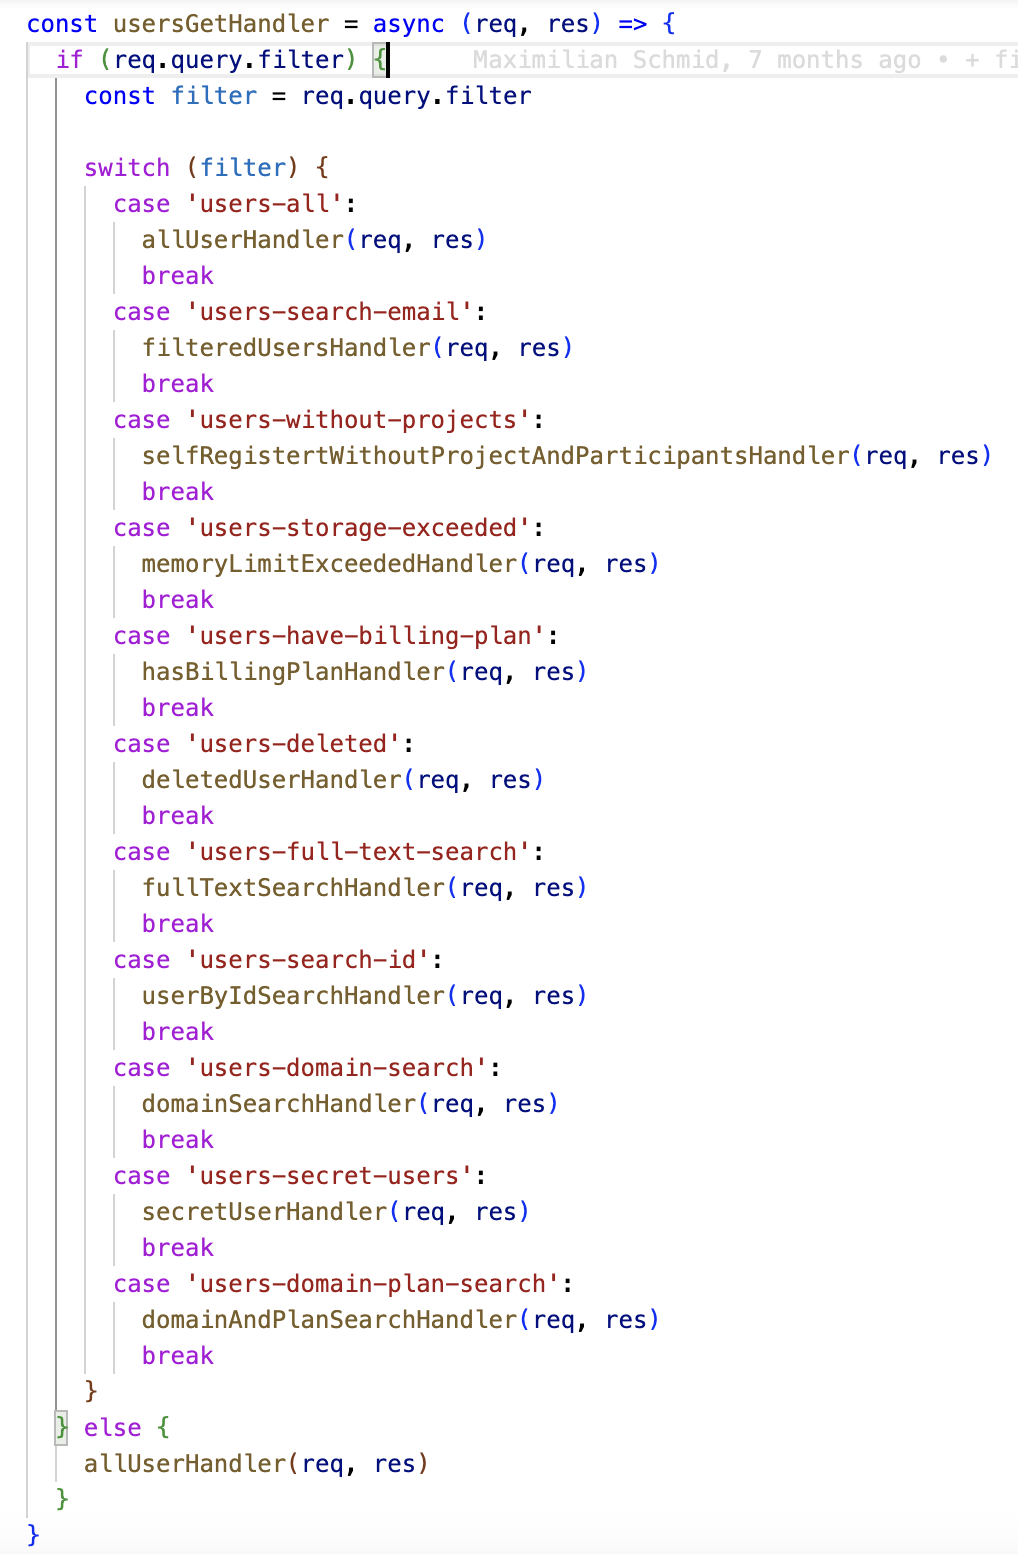
\includegraphics[width=0.6\textwidth]{pics/REST_API_Img.png}
    \caption{User-GET-Handler}
    \label{fig:enter-label}
\end{figure}